\chapter{Die Synthese-Pipeline}
\label{kap:pipeline}

Dieses Kapitel dokumentiert die Pipeline, die aus neun Objektausschnitten und
sieben Hintergrundaufnahmen den vollständigen Trainingsdatensatz erzeugt. Für
jede Transformation werden der Parameterbereich, der \emph{gemessene} Anteil im
erzeugten Datensatz und die Begründung angegeben. Die Anteile sind keine
konfigurierten Sollwerte, sondern Ist-Werte aus dem Erzeugungsbericht
\code{synth/train/generation\_report.json} über 6000 Bilder mit 173\,100
gerenderten Instanzen und 136\,384 gelabelten Objekten. Wo Soll- und Ist-Wert
auseinanderfallen, ist dies erklärbar und wird erklärt.

\section{Leitprinzip und Arbeitsteilung}
\label{sec:leitprinzip}

\absatz{Leitprinzip.} Die Pipeline verfolgt genau ein Ziel: \emph{jede Abkürzung
schließen, über die ein CNN \enquote{hier wurde etwas eingeklebt} statt
\enquote{hier ist ein Rohrende} lernen könnte.} Wie in
Abschnitt~\ref{sec:shortcut} begründet, ist bei Copy-Paste-Synthese nicht zu
wenig Variation die dominante Fehlerquelle, sondern der systematische Unterschied
zwischen eingefügten und originalen Pixeln. Jede Transformation wird deshalb
entweder mit einer Messung an den Realdaten (Kapitel~\ref{kap:daten}), mit einer
physikalischen Randbedingung oder mit einer konkret benannten Abkürzung
begründet, die sie schließt.

\absatz{Arbeitsteilung Generator / Trainingszeit.} Das zweite Prinzip folgt
unmittelbar aus Anforderung~A1 (Labelexaktheit). Transformationen werden dort
ausgeführt, wo ihre Labeltransformation exakt bekannt ist:

\begin{table}[htbp]
\centering
\caption[Arbeitsteilung Generator und Trainingszeit]{Arbeitsteilung zwischen
Generator (offline) und Trainingszeit-Augmentierung. Kriterium ist
ausschließlich, ob die Labeltransformation exakt bekannt ist.}
\label{tab:arbeitsteilung}
\small
\begin{tabularx}{\textwidth}{@{}L{0.42\textwidth}X@{}}
\toprule
\textbf{Generator (offline, pro Instanz)} &
\textbf{Trainingszeit (Ultralytics, bildweit)} \\
\midrule
Alles, was \emph{pro Instanz} wirkt und die Box aus der transformierten
Alphamaske \emph{exakt neu} bestimmt: Rotation über den vollen Kreis,
Ovalisierung, Delle, Perspektive, Photometrie, Verdeckung, Sichtbarkeitsrechnung &
Alles, was \emph{bildweit} wirkt und Boxen nicht verfälscht: Mosaic,
Skalierung, Translation, Spiegelung, HSV-Variation \\
\bottomrule
\end{tabularx}
\end{table}

Aus dieser Aufteilung folgt zwingend, dass im Training \code{degrees=0},
\code{shear=0} und \code{perspective=0} gesetzt sind: Diese Operationen blähen
achsparallele Boxen auf (Abschnitt~\ref{sec:boxrotation}). Im Generator dagegen
wird die Box nach der Rotation aus der gedrehten Alphamaske neu bestimmt und ist
damit exakt. Die genannten Invarianzen werden also nicht \emph{weggelassen},
sondern nur an einer anderen Stelle -- und label-exakt -- erzeugt.

\begin{figure}[htbp]
\centering
\begin{tikzpicture}[
  box/.style={draw,rounded corners=2pt,align=center,font=\scriptsize,
              text width=1.85cm,minimum height=8.5mm,inner sep=2.5pt,fill=blue!8},
  stage/.style={draw,rounded corners=2pt,align=center,font=\scriptsize,
              text width=1.85cm,minimum height=9.5mm,inner sep=2.5pt,fill=orange!18},
  erg/.style={draw,rounded corners=2pt,align=center,font=\scriptsize,
              text width=2.1cm,minimum height=9.5mm,inner sep=2.5pt,fill=green!12},
  ar/.style={-{Latex[length=1.8mm]},semithick,gray!60!black}]
  \node[box]   (cut)   at (0,1.25)  {9 Objekt-\\ausschnitte};
  \node[box]   (bg)    at (0,-1.25) {7 Hintergrund-\\aufnahmen};
  \node[stage] (mat)   at (2.9,1.25) {\textbf{Stufe 1}\\Matting};
  \node[stage] (occ)   at (2.9,-1.25){\textbf{Stufe 2}\\Okkluder};
  \node[box]   (masks) at (5.7,1.25) {9 Alphamasken\\(1{,}1\,px Kante)};
  \node[box]   (bars)  at (5.7,-1.25){56 echte\\Rohrschäfte};
  \node[stage] (syn)   at (8.6,0)    {\textbf{Stufe 3}\\Synthese\\T1--T9};
  \node[erg]   (ds)    at (11.6,0)   {6000 Bilder\\136\,384 Labels};
  \draw[ar] (cut) -- (mat);
  \draw[ar] (bg)  -- (occ);
  \draw[ar] (mat) -- (masks);
  \draw[ar] (occ) -- (bars);
  \draw[ar] (masks) -- (syn);
  \draw[ar] (bars)  -- (syn);
  \draw[ar] (bg.south) -- ++(0,-0.7) -| (syn.south);
  \draw[ar] (syn) -- (ds);
  \node[font=\scriptsize,gray!50!black,fill=white,inner sep=1.5pt]
        at (4.1,-2.35) {Hintergründe zusätzlich direkt};
\end{tikzpicture}
\caption[Aufbau der Pipeline]{Aufbau der Pipeline. Die Hintergrundaufnahmen
werden zweifach genutzt: als Quelle der Okkluder-Bibliothek (Stufe~2) und
unmittelbar als Bildhintergrund und Fremdkörperquelle (Stufe~3).}
\label{abb:pipeline}
\end{figure}

\section{Stufe 1 -- Freistellen der Objektausschnitte}
\label{sec:matting}

\absatz{Problem.} Nach Befund~1 sind alle neun Ausschnitte rechteckig, 13--35\,\%
ihrer Fläche ist Fremdkontext. Direktes Einkopieren erzeugt Signatur~S1.

\absatz{Lösung.} Das Freistellen erfolgt dreistufig über ein Ellipsenmodell
$(c_x, c_y, r_x, r_y, \theta)$ pro Ausschnitt:

\begin{enumerate}
  \item \textbf{Manuelle Startwerte}, abgelesen aus einer 14-fach vergrößerten
  Rasteransicht. Bei neun Objekten ist das exakter als jeder automatische Fit und
  vermeidet, dass ein Fehlschlag der Optimierung unbemerkt bleibt.
  \item \textbf{Numerische Verfeinerung} per Coordinate Descent. Maximiert wird
  die radiale Kantenenergie $I(\text{innen}) - I(\text{außen})$ entlang der
  Ellipse auf einem sechsfach upgesampelten, geglätteten Bild. Das Upsampling ist
  nötig, weil die Objekte nur 28--43\px{} groß sind und eine Verschiebung um ein
  Pixel bereits mehrere Prozent des Radius ausmacht.
  \item \textbf{Außenkantenkorrektur.} Schritt~2 konvergiert
  konstruktionsbedingt auf den \emph{Grat} des hellen Kranzes, nicht auf seine
  Außenkante. Ein mittleres Radialprofil bestimmt daher zusätzlich den Radius,
  bei dem die Helligkeit auf 25\,\% der Kantenamplitude über Hintergrundniveau
  abgefallen ist.
\end{enumerate}

\absatz{Warum 25\,\% und nicht 50\,\%?} Der klassische Schwellwert für eine
Kantenposition ist der Halbwertspunkt (FWHM-Konvention, \cite{gonzalez2018}). Die
Wahl von 25\,\% verschiebt die Maskengrenze bewusst nach außen. Die Begründung
ist asymmetrisch in den Kosten: Der helle Kranz ist das \emph{diskriminative}
Merkmal des Objekts -- ihn anzuschneiden entfernt Information, die das Netz
braucht. Ein etwa 1\px{} breiter Hintergrundsaum dagegen wird durch das
anschließende Feathering und den Farbangleich (Abschnitt~\ref{sec:photometrie})
ohnehin kaschiert. Die Aufweitung wird hart auf $[1{,}02;\,1{,}10]$ gedeckelt:
Bei acht der neun Ausschnitte liegt der ermittelte Faktor bei 1,02--1,05; nur der
kontrastarme \code{cutted\_8.png} liefe sonst auf 1,19 und die Maske würde
Hintergrund aufsaugen.

\absatz{Ergebnis.} Weiche Alphamasken mit rund 1,1\px{} Übergangsbreite
(Abbildung~\ref{abb:matting}). Der weiche Übergang ist Absicht und nicht
Toleranz: Ein 25\px{} großes Objekt hat in einer echten Aufnahme nie eine
pixelharte Silhouette, weil Objektivunschärfe und Sensortiefpass jede Kante über
mindestens ein Pixel verschmieren.

\begin{figure}[htbp]
\centering
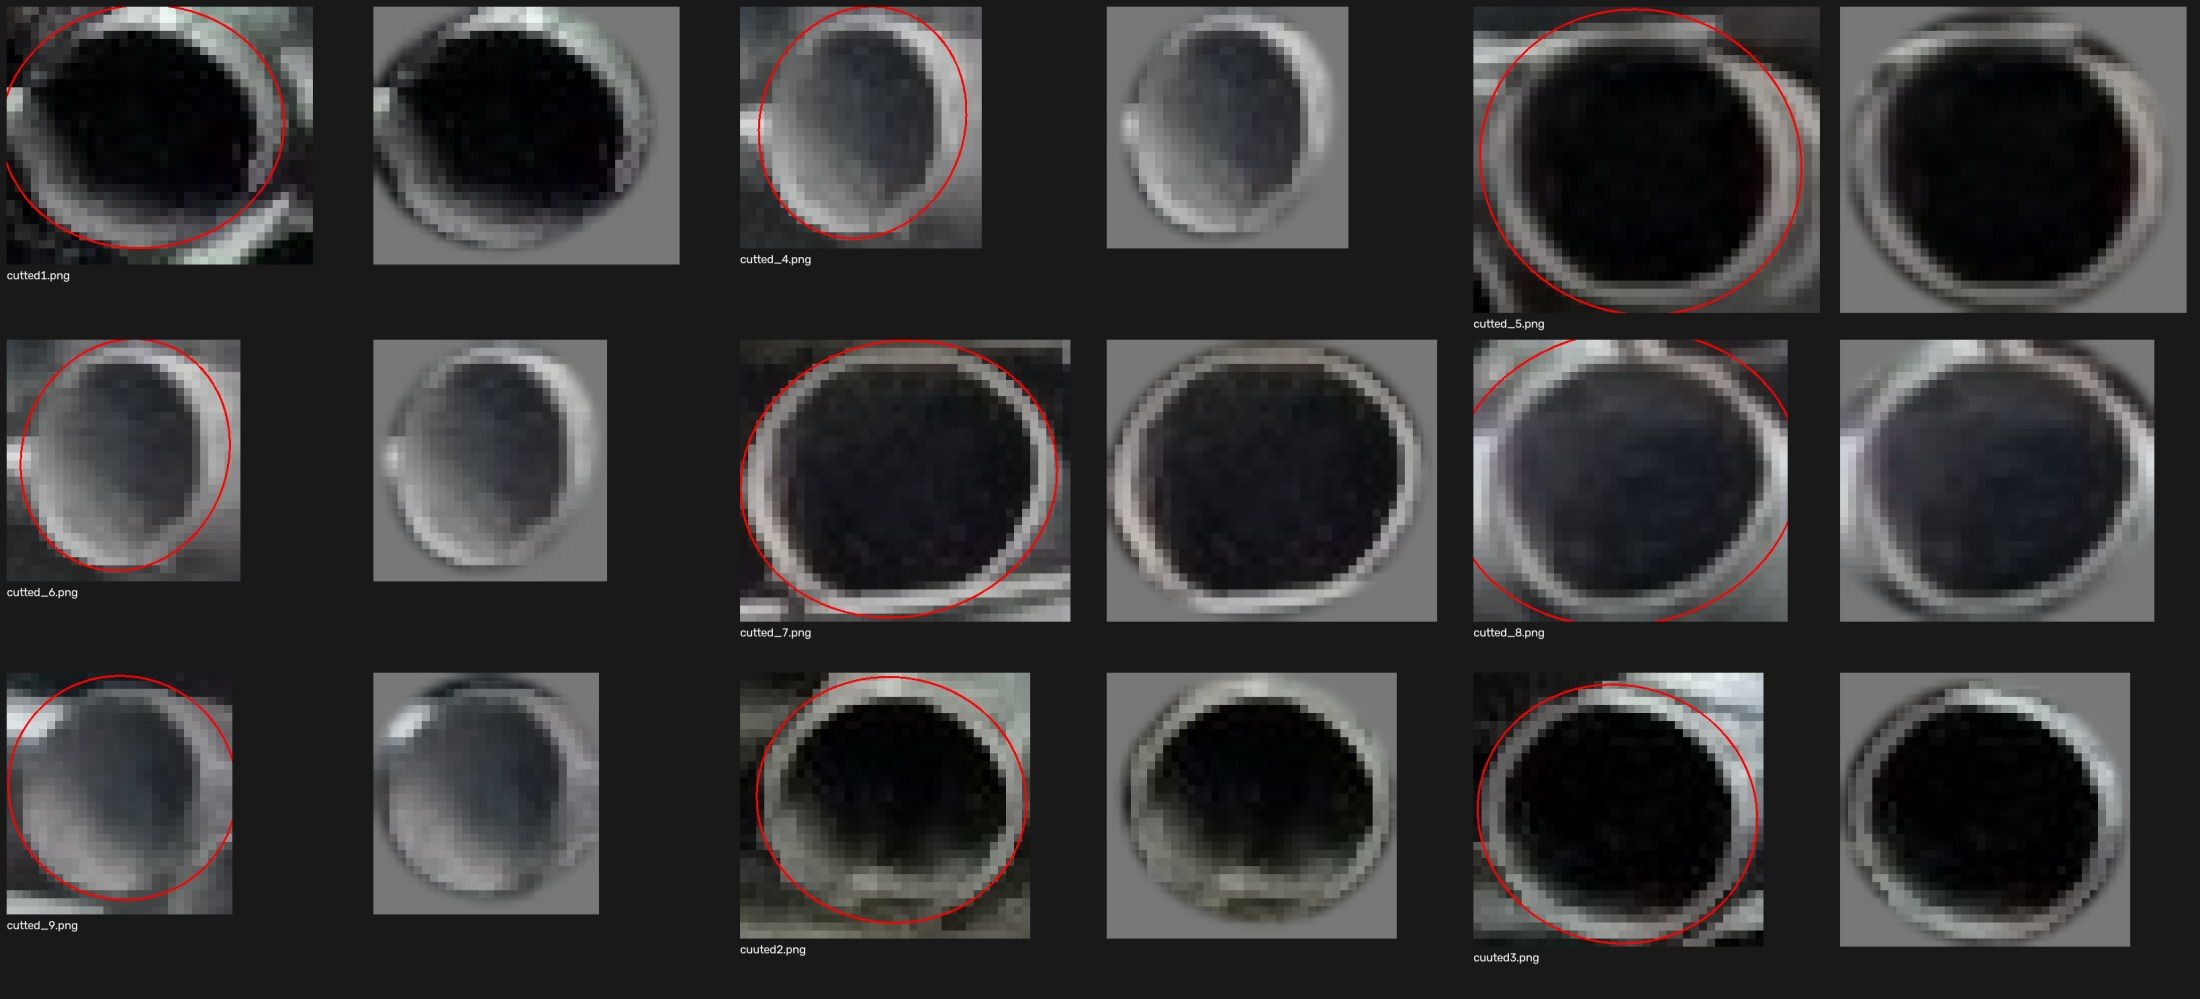
\includegraphics[width=\textwidth]{abbildungen/matting_check.jpg}
\caption[Kontrolle des Freistellens]{Kontrolle des Freistellens für alle neun
Ausschnitte. Je Paar links das Original mit eingezeichneter Ellipse, rechts das
freigestellte Objekt auf neutralem Grau. Erkennbar ist die weiche Kante und der
bewusst außen liegende Maskenrand, der den hellen Kranz vollständig einschließt.}
\label{abb:matting}
\end{figure}

\section{Stufe 2 -- Okkluder-Bibliothek}
\label{sec:okkluderbib}

\absatz{Warum echte Rohrschäfte statt gezeichneter Balken.} Verdeckung liegt in
der Zieldomäne durch quer liegende Rohre vor. Ein synthetisch \emph{gemalter}
Balken hätte andere Textur-, Rausch- und Glanzstatistik als der Rest des Bildes
-- das Netz könnte \enquote{Objekt liegt neben künstlichem Balken} lernen, also
eine Abkürzung der Klasse S2--S4. Die vier Clean Plates sind dagegen buchstäblich
Wände aus Rohrschäften desselben Materials, derselben Kamera und derselben
Beleuchtung. Aus ihnen lassen sich Okkluder gewinnen, deren
Sensorsignatur identisch ist.

\absatz{Verfahren.}
\begin{enumerate}
  \item Bestimmung der dominanten Rohrrichtung über den \textbf{Struktur-Tensor}
  \parencite{jaehne2005}, Winkel auf $(-45^\circ, 45^\circ]$ gefaltet, Bild
  entsprechend gedreht. Gemessen: $+0{,}9^\circ$, $-1{,}6^\circ$,
  $+0{,}9^\circ$, $+6{,}6^\circ$.
  \item Zeilenmittelprofil des gedrehten Bildes, Hochpassfilterung, lokale
  Maxima als \textbf{Rohrachsen}; ihr mittlerer Abstand ist der Rohrdurchmesser.
  Gemessen: 16, 18, 21, 20\px{} -- dieselben Werte, die
  Tabelle~\ref{tab:hintergruende} als Maßstabsanker nennt.
  \item Ausschneiden eines Streifens der Höhe = Achsabstand um jede Achse.
  \item Weiche \textbf{Kapselmaske} (Rechteck mit halbrunden Enden, 1,6\px{}
  Feder), damit die Schaftenden nicht als gerade Schnittkante enden.
\end{enumerate}

\absatz{Ergebnis.} 56 Rohrschäfte mit echter zylindrischer Schattierung und
echtem Glanzlicht (Abbildung~\ref{abb:okkluder}). Sie werden in der Synthese
zweifach verwendet: als Schaft \emph{hinter} jeder Stirnfläche
(Abschnitt~\ref{sec:schaft}) und als quer liegender Okkluder \emph{vor} dem
Stapel (Abschnitt~\ref{sec:okklusion}).

\begin{figure}[htbp]
\centering
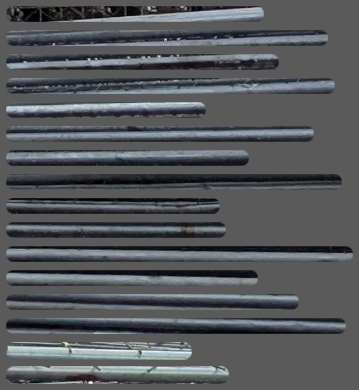
\includegraphics[width=0.42\textwidth]{abbildungen/okkluder_check.png}
\caption[Okkluder-Bibliothek]{Ausschnitt aus der Okkluder-Bibliothek: aus den
Clean Plates extrahierte echte Rohrschäfte mit zylindrischer Schattierung,
Glanzlicht und weicher Kapselmaske.}
\label{abb:okkluder}
\end{figure}

\section{Stufe 3 -- Bildsynthese}
\label{sec:synthese}

Die Leinwand ist $1024\times1024$ Pixel groß und damit identisch zur
Trainingsauflösung \code{imgsz=1024}. Das ist eine bewusste Entscheidung nach
Anforderung~A2: Die synthetischen Bilder durchlaufen im Training \emph{keine}
Größenänderung, die sorgfältig kalibrierte Objektgrößenverteilung bleibt exakt
erhalten.

\subsection{T1 -- Hintergrund}
\label{sec:hintergrundstufe}

\begin{table}[htbp]
\centering
\caption[T1: Hintergrundstufe]{T1 -- Hintergrundstufe. \emph{Ist} = gemessener
Anteil je Bild im erzeugten Datensatz. Belegart wie in
Tabelle~\ref{tab:mapping}.}
\label{tab:t1}
\footnotesize
\begin{tabularx}{\textwidth}{@{}L{0.20\textwidth}L{0.10\textwidth}XL{0.045\textwidth}@{}}
\toprule
\textbf{Transformation} & \textbf{Ist} & \textbf{Begründung} & \textbf{Art} \\
\midrule
Clean Plate statt Fremdszene & 80\,\% (Soll) &
Die vier Clean Plates sind exakt die Zieldomäne und erhalten sechsfaches
Ziehgewicht. Die drei Fremdszenen liefern zu 20\,\% Kontextvielfalt und harte
Negative -- \code{bg\_5.jpg} enthält den Maschendraht, der nach der
Annotationsdefinition kein Objekt ist. & M \\
Zoom gekoppelt an den Rohrdurchmesser & 100\,\% &
\textbf{Physikalische Randbedingung} (Befund~6). Statt Zoom und Objektgröße
unabhängig zu ziehen, gilt $d = d_{\text{Rohr}}(\text{bg}) \cdot z$. Ein
Missverhältnis zwischen Stirnfläche und benachbartem Schaft wäre physikalisch
unmöglich und trainierte eine falsche Kontext-Größen-Relation an. & P \\
Zufallsausschnitt (Translation) & 100\,\% &
Verhindert, dass immer derselbe Bildbereich als Hintergrund dient -- bei nur
sieben Quellbildern die wichtigste Quelle von Hintergrundvielfalt. & L \\
Reflect-Padding statt Kachelung & nach Bedarf &
Wird der geforderte Ausschnitt größer als das Quellbild, so wird gespiegelt
aufgefüllt, gedeckelt auf $1{,}35 \times$ kürzeste Kante. \code{np.tile} erzeugte
harte achsparallele Nähte (S1); gespiegeltes Padding hat keine Kante. & L \\
Horizontale Spiegelung & 50{,}5\,\% &
Label-exakt und physikalisch korrekt: Ein Stapel wird von beiden Enden
fotografiert. & P \\
Vertikale Spiegelung & 14{,}9\,\% &
Ebenfalls label-exakt. Bewusst seltener als horizontal, weil die Schwerkraft
(Stapel unten, Himmel oben) eine schwache Vorzugsrichtung erzeugt. & A \\
Kleinrotation $\pm 6^\circ$ & 34{,}3\,\% &
Die Rohrlinien im Bild sind nie exakt achsparallel; ohne diese Variation wäre
die Vorzugsrichtung im Datensatz künstlich diskret. Angewandt \emph{vor} dem
Einfügen der Objekte, betrifft also keine Boxen. Begleitender Zoom 1,06 gegen
Eckartefakte. & M \\
\bottomrule
\end{tabularx}
\end{table}

Der Zoomfaktor $z$ wird so gezogen, dass der resultierende Basisdurchmesser im
Zielbereich $[d_{\min}, d_{\max}] = [12, 44]$\px{} liegt:
\begin{equation}
z \sim \mathcal{U}\!\left[\;\max\!\left(0{,}55,\;
\frac{d_{\min}}{d_{\text{Rohr}}}\right),\;
\min\!\left(2{,}20,\;\frac{d_{\max}}{d_{\text{Rohr}}}\right)\right],
\qquad d_{\text{Basis}} = d_{\text{Rohr}} \cdot z .
\label{eq:zoom}
\end{equation}
Die äußeren Schranken 0,55 und 2,20 begrenzen die Vergrößerung des
Hintergrundmaterials und damit den Verlust an Hintergrundschärfe. Für
$d_{\text{Rohr}} = 16$\px{} ergibt Gleichung~\eqref{eq:zoom}
$z \in [0{,}75;\,2{,}20]$, für $d_{\text{Rohr}} = 21$\px{}
$z \in [0{,}57;\,2{,}10]$. Der Ausschnitt der Kantenlänge $1024/z$ wird
anschließend auf die Leinwand skaliert -- beim Verkleinern flächentreu
(\code{INTER\_AREA}), um Aliasing zu vermeiden (S3).

\subsection{T2 -- Geometrie der Einzelinstanz}
\label{sec:instanzgeometrie}

\begin{table}[htbp]
\centering
\caption[T2: Instanzgeometrie]{T2 -- Geometrie der Einzelinstanz. \emph{Ist} =
gemessener Anteil je gerenderter Instanz.}
\label{tab:t2}
\footnotesize
\begin{tabularx}{\textwidth}{@{}L{0.19\textwidth}L{0.11\textwidth}XL{0.045\textwidth}@{}}
\toprule
\textbf{Transformation} & \textbf{Ist} & \textbf{Begründung} & \textbf{Art} \\
\midrule
Rotation $0$--$360^\circ$ & 100\,\% &
Rohrenden haben keine kanonische Bildorientierung: Kamerarollwinkel und
Stapelausrichtung sind beliebig. Die einzige Orientierungsinformation ist die
Richtung des Glanzlichts auf dem Kranz, und die hängt vom Sonnenstand ab. Volle
Rotationsinvarianz ist daher korrekt \emph{und kostenlos} -- es gibt keine
Rotation, die ein unmögliches Bild erzeugt. Deshalb 100\,\% statt eines
Bruchteils. & P \\
Skalierung auf 12--44\px{} & 100\,\% &
Reale Messung (Tabelle~\ref{tab:objektstatistik}): \code{val} 20,6--35,8\px{},
\code{test} 12,2--31,9\px{}. Der Generator deckt die reale Spanne plus rund
25\,\% Reserve nach oben ab, für Aufnahmen aus geringerem Abstand.
Ist-Verteilung im Datensatz: p05 11,6 / Median 22,5 / p95 39,9\px{}.
Verkleinerung flächentreu, weil bilineare Interpolation Aliasing als
verräterisches Hochfrequenzmuster im Objekt zurückließe (S3). & M \\
Ovalisierung & 57{,}1\,\% &
Reale Messung: Seitenverhältnis p10--p90 = 0,97--1,31 (\code{val}) bzw.\
0,85--1,22 (\code{test}); über die Hälfte der echten Boxen weicht um
$\geq 5\,\%$ vom Quadrat ab. Zwei physikalische Ursachen: Schrägansicht
projiziert den Kreis auf eine Ellipse, und Rohre sind tatsächlich gequetscht.
Der Anteil bildet die gemessene Häufigkeit ab. Aufteilung 45\,\% oblat
(0,66--0,97) zu 12\,\% prolat (1,03--1,30), weil Schrägansicht die Höhe
verkürzt und häufiger ist als eine seitliche Quetschung. & M \\
Delle & 18{,}1\,\% &
Modelliert mechanisch beschädigte Rohrenden. \textbf{Der Anteil ist eine
Annahme, keine Messung} -- Dellen sind in \code{val}/\code{test} nicht separat
annotiert. 18\,\% wurde gewählt, damit das Modell die Verformung regelmäßig
sieht (etwa jedes fünfte Objekt, im Mittel vier pro Bild), sie aber die
Formstatistik nicht dominiert. Ein zu hoher Anteil würde die Rundheit als
Merkmal verwässern und Falschpositive auf beliebigen dunklen Flecken erzeugen
(vgl.\ Abschnitt~\ref{sec:auggrenzen}). & A \\
Perspektive & 30{,}2\,\% &
Bei Schrägblick wird der Kreisring nicht nur zur Ellipse -- der helle Kranz wird
auf einer Seite auch \emph{breiter}, weil die Rohrinnenwand sichtbar wird. Eine
rein anisotrope Skalierung kann das nicht abbilden. Der Anteil ist eine Annahme;
30\,\% spiegelt die Beobachtung, dass in \code{val}/\code{test} die Mehrheit der
Stirnflächen annähernd frontal steht. & A \\
\bottomrule
\end{tabularx}
\end{table}

\absatz{Skalierung und Ovalisierung.} Beide werden in einem Schritt ausgeführt.
Ist $d_{\text{src}}$ der Durchmesser des Quellausschnitts, $d$ der Zieldurchmesser
und $\rho$ das gezogene Achsverhältnis, so gilt
\begin{equation}
s_x = \frac{d}{d_{\text{src}}\sqrt{\rho}}, \qquad
s_y = \frac{d\,\sqrt{\rho}}{d_{\text{src}}} .
\label{eq:oval}
\end{equation}
Der geometrische Mittelwert bleibt dabei erhalten:
$\sqrt{s_x s_y}\, d_{\text{src}} = d$. Das ist kein Zufall, sondern notwendig,
damit die Ovalisierung die kalibrierte Größenverteilung nicht verschiebt -- die
Realmessung in Tabelle~\ref{tab:objektstatistik} verwendet mit
$\sqrt{\text{Fläche}}$ genau dieses Maß.

\absatz{Dellenmodell.} Die Einbeulung wird als glatte radiale Verschiebung
umgesetzt. Für $K \in \{1,2\}$ Winkelsektoren mit Mittelrichtungen $\varphi_k$,
Breiten $\sigma_k \sim \mathcal{U}[0{,}30;\,0{,}85]$\,rad und
Eindringtiefen $a_k \sim \mathcal{U}[0{,}10;\,0{,}30]$ lautet das
Verschiebungsfeld in Polarkoordinaten um den Objektmittelpunkt
\begin{equation}
u(r, \varphi) = \sum_{k=1}^{K} a_k
\exp\!\left(-\left(\frac{\Delta\varphi_k}{\sigma_k}\right)^{2}\right)
\left(\frac{r}{R}\right)^{2},
\qquad \Delta\varphi_k = \operatorname{atan2}\!\big(\sin(\varphi-\varphi_k),
\cos(\varphi-\varphi_k)\big),
\label{eq:delle}
\end{equation}
und die Abtastung erfolgt an $r \cdot (1 + u)$. Die quadratische Radiusgewichtung
$(r/R)^2$ ist der wesentliche Modellierungsentscheid: Sie hält das Zentrum ruhig
und verformt nur den Rand. Eine gleichmäßige Verschiebung würde die dunkle
Bohrung mitverzerren und damit das Merkmalspaar Kranz/Bohrung zerstören, statt
nur den Umriss zu beschädigen.

\absatz{Perspektive.} Umgesetzt als milde Homographie: Die vier Eckpunkte des
Instanzausschnitts werden unabhängig um bis zu $\pm 9\,\%$ der Kantenlänge
verschoben. Der Wert 9\,\% ist so gewählt, dass die entstehende Verzerrung
sichtbar, aber nicht mit einer Schrägansicht von mehr als etwa $25^\circ$
verwechselbar ist -- stärkere Verzerrungen kämen bei einer frontal auf den
Stapel gerichteten Kamera nicht vor.

\absatz{Rotation.} Die Instanz wird auf eine quadratische Leinwand der Größe
ihrer Diagonale erweitert und um $\theta \sim \mathcal{U}[0^\circ, 360^\circ]$
gedreht. Die Box wird anschließend nicht aus $\theta$ berechnet, sondern aus der
gedrehten Alphamaske selbst -- damit entfällt die in
Abschnitt~\ref{sec:boxrotation} beschriebene Aufblähung vollständig
(Anforderung~A1).

\subsection{T3 -- Photometrie und Einbettungsrealismus}
\label{sec:photometrie}

Diese Stufe schließt die Signaturen S2--S4 und S6. Sie ist der aufwendigste Teil
der Pipeline und derjenige, dessen Wirkung optisch am wenigsten auffällt.

\begin{table}[htbp]
\centering
\caption[T3: Photometrie und Einbettungsrealismus]{T3 -- Photometrie der
Einzelinstanz und Einbettungsrealismus. \emph{Ist} = gemessener Anteil je
gerenderter Instanz. Die Spalte \emph{S} nennt die geschlossene Abkürzung aus
Abschnitt~\ref{sec:shortcut}.}
\label{tab:t3}
\footnotesize
\begin{tabularx}{\textwidth}{@{}L{0.19\textwidth}L{0.07\textwidth}L{0.035\textwidth}XL{0.045\textwidth}@{}}
\toprule
\textbf{Transformation} & \textbf{Ist} & \textbf{S} & \textbf{Begründung} & \textbf{Art} \\
\midrule
Helligkeit $\times 0{,}70$--$1{,}35$ & 99{,}8\,\% & -- &
Stirnflächen liegen je nach Stapelposition in praller Sonne oder tiefem
Schatten. Die Spannweite ist aus den Ausschnitten selbst ablesbar: mittlere
Kranzhelligkeit 88--156 Grauwerte. Praktisch 100\,\%, weil es keine
\enquote{richtige} Helligkeit gibt, die bevorzugt werden dürfte. & M \\
Gamma $0{,}75$--$1{,}35$ & 79{,}7\,\% & -- &
Gamma statt reinem Kontrast, weil es die nichtlineare Tonwertkurve
unterschiedlicher Kameras und JPEG-Pipelines abbildet
\parencite{grossberg2003}. Es verändert vor allem das Verhältnis dunkle Bohrung
$\leftrightarrow$ heller Kranz -- genau das Merkmal, auf das der Detektor sonst
zu starr konditioniert würde. & L \\
HSV (Ton $\pm 8^\circ$, Sättigung $\times 0{,}45$--$1{,}60$) & 69{,}7\,\% & -- &
Verzinkter Stahl ist nahezu neutralgrau, nimmt aber Farbstiche an: Flugrost
braun, Moos grün, blauer Himmel als Reflex. Der Farbtonhub ist bewusst klein --
große Sprünge wären unphysikalisch. & M \\
Farbangleich an den lokalen Hintergrund & 84{,}8\,\% & S2 &
\textbf{Die wichtigste Anti-Abkürzungs-Maßnahme.} Ausschnitt und Hintergrund
stammen aus verschiedenen Aufnahmen mit verschiedenem Weißabgleich und
Belichtungsniveau; ohne Angleich bleibt ein konstanter Versatz, den ein CNN
trivial als Einfügemarke lernt. Bewusst nur \emph{teilweise}
(Gleichung~\eqref{eq:harmonize}). & L \\
Unschärfeangleich ($\sigma$ 0,25--1,10\px) & 59{,}8\,\% & S3 &
Zwei Gründe: Das skalierte Objekt ist je nach Skalierungsrichtung glatter oder
schärfer als das Zielbild, und reale Objekte liegen je nach Stapeltiefe
außerhalb der Schärfeebene. Schärfe ist eine der beiden Sensorsignaturen, an
denen eingeklebte Pixel am leichtesten erkennbar sind
\parencite{popescu2005}. & L \\
Rauschangleich ($\times 0{,}5$--$1{,}25$ der lokalen Schätzung) & 69{,}9\,\% & S4 &
Die zweite Sensorsignatur \parencite{lukas2006}. Beim Verkleinern eines
Ausschnitts sinkt dessen Rauschen; der eingeklebte Bereich wäre dann messbar
sauberer als seine Umgebung. Das Rauschniveau wird \emph{pro Einfügestelle
gemessen} (Gleichung~\eqref{eq:noise}), nicht global gesetzt -- die Hintergründe
liegen zwischen 6,8 und 15,2 Grauwerten Hochpassstreuung. & L \\
Alphakante weichzeichnen ($\sigma$ 0,4--1,0\px) & 100\,\% & S1 &
Immer. Eine pixelharte Silhouette gibt es bei 25\px{}-Objekten in echten
Aufnahmen nicht. & P \\
Schlagschatten & 49{,}3\,\% & S6 &
Ohne Kontaktschatten \enquote{schwebt} ein eingeklebtes Objekt sichtbar. Rund
50\,\%, weil bei diffusem Licht -- alle vier Clean Plates sind bedeckt
aufgenommen -- etwa die Hälfte der realen Objekte keinen sichtbaren
Schlagschatten wirft. & A \\
\bottomrule
\end{tabularx}
\end{table}

\absatz{Farbangleich.} Umgesetzt als \emph{partieller} Statistiktransfer im Stil
des Farbtransfers von \textcite{reinhard2001}. Für jeden Farbkanal $c$ seien
$\mu_i, \sigma_i$ Mittelwert und Streuung der Objektpixel (Alphamaske $> 0{,}5$)
und $\mu_b, \sigma_b$ dieselben Größen des lokalen Hintergrundausschnitts. Dann
gilt
\begin{equation}
c' = \mu_i + k\,(c - \mu_i) + \alpha_\mu\,(\mu_b - \mu_i),
\qquad
k = 1 + \alpha_\sigma\left(\operatorname{clip}\!\left(
\frac{\sigma_b}{\sigma_i},\, 0{,}6,\, 1{,}6\right) - 1\right)
\label{eq:harmonize}
\end{equation}
mit $\alpha_\mu \sim \mathcal{U}[0{,}10;\,0{,}45]$ und
$\alpha_\sigma \sim \mathcal{U}[0;\,0{,}35]$. Für
$\alpha_\mu = \alpha_\sigma = 1$ ginge Gleichung~\eqref{eq:harmonize} in den
vollständigen Reinhard-Transfer über. Genau das ist hier \emph{nicht} gewollt:
Ein vollständiger Angleich würde den intrinsischen Albedo-Unterschied zwischen
dunkler Bohrung und hellem Kranz einebnen und damit das Objekt zerstören.
Modelliert wird also ausschließlich die \emph{Beleuchtungs- und
Weißabgleichdifferenz} zwischen den Aufnahmen, nicht die Objektfarbe. Die
Klemmung des Streuungsverhältnisses auf $[0{,}6;\,1{,}6]$ verhindert
Ausreißer an Einfügestellen mit sehr homogenem Hintergrund, wo
$\sigma_b/\sigma_i$ beliebig klein werden kann.

\absatz{Rauschschätzung.} Das lokale Rauschniveau wird als Streuung eines
Hochpassrests geschätzt -- ein Verfahren in der Tradition von
\textcite{immerkaer1996}, hier mit einem Medianfilter als Tiefpass, weil er
Kanten weniger verschmiert als ein Gaußkern:
\begin{equation}
\hat{\sigma} = \operatorname{std}\!\big(g - \operatorname{median}_{3\times3}(g)\big),
\qquad
\sigma_{\text{Rausch}} = \max\big(0{,}5,\; \hat{\sigma} \cdot
\mathcal{U}[0{,}5;\,1{,}25]\big).
\label{eq:noise}
\end{equation}
Die Multiplikation mit einem Faktor um 1 statt der direkten Verwendung von
$\hat\sigma$ ist Absicht: Die Schätzung enthält neben dem Rauschen auch
Texturanteile und überschätzt das Niveau an strukturreichen Stellen.

\absatz{Schlagschatten.} Die Alphamaske wird mit $\sigma = 0{,}10 \cdot
\max(h,w)$ geglättet, um $\Delta x \sim \mathcal{U}[-0{,}22;\,0{,}22]\,w$ und
$\Delta y \sim \mathcal{U}[0{,}02;\,0{,}26]\,h$ verschoben und die Leinwand dort
um den Faktor $1 - \kappa\,s$ mit $\kappa \sim \mathcal{U}[0{,}18;\,0{,}45]$
abgedunkelt. Der Versatz ist in $y$ ausschließlich positiv: Bei einer von unten
oder frontal aufgenommenen Szene mit Himmelslicht fällt der Kontaktschatten nach
unten.

\subsection{T4 -- Layout}
\label{sec:layout}

Das Layoutmodell ist eine \textbf{gescherte, verrauschte Gitterpackung} je
Cluster. Pro Bild werden 1--3 Cluster gezogen (Anteile 45/35/20\,\%), dazu 0--3
vereinzelte Profile. Innerhalb eines Clusters mit Basisdurchmesser $d_0$ liegen
die Zentren auf
\begin{equation}
p_{ij} = i\,s_1\,\mathbf{e}_1 + j\,s_2\,\mathbf{e}_2 + \mathbf{c}
+ \boldsymbol{\epsilon}_{ij},
\qquad \boldsymbol{\epsilon}_{ij} \sim \mathcal{N}(\mathbf{0},
(0{,}17\,d_0)^2 \mathbf{I}),
\label{eq:layout}
\end{equation}
mit $i = 0,\dots,n_1{-}1$, $j = 0,\dots,n_2{-}1$,
$n_1 \in \{2,\dots,13\}$, $n_2 \in \{1,\dots,6\}$, Gitterabständen
$s_1 \sim \mathcal{U}[0{,}98;\,1{,}60]\,d_0$ und
$s_2 \sim \mathcal{U}[0{,}98;\,1{,}85]\,d_0$ sowie Basisrichtungen
$\mathbf{e}_1, \mathbf{e}_2$, die einen Winkel zwischen $55^\circ$ und
$125^\circ$ einschließen. Die Hauptrichtung liegt mit Wahrscheinlichkeit 0,6 im
Bereich $60$--$150^\circ$, sonst gleichverteilt -- das bildet die in
Tabelle~\ref{tab:anordnung} gemessene leichte Häufung der Nachbarrichtungen ab,
ohne sie zu einer harten Regel zu machen.

Zwei Modellentscheidungen folgen unmittelbar aus den Messungen:

\begin{itemize}
  \item \textbf{Eine Basisgröße pro Cluster}, je Instanz nur
  $\mathcal{U}[0{,}92;\,1{,}09]$ Streuung. Begründung: Befund~8 (gemessenes
  Größenverhältnis benachbarter Objekte im Median 1,05). Jede Instanz unabhängig
  zu würfeln wäre ein sofort sichtbarer Realismusfehler.
  \item \textbf{Das Clusterzentrum darf außerhalb der Leinwand liegen}
  ($\mathbf{c} \sim \mathcal{U}[-0{,}12;\,1{,}12]^2 \cdot 1024$), sodass
  angeschnittene Objekte am Bildrand entstehen. Begründung: In \code{test} sind
  5,8\,\% der Labels angeschnitten.
\end{itemize}

\absatz{Abgedunkelte Mulde.} Zusätzlich wird je Cluster mit Wahrscheinlichkeit
0,55 eine weiche, anisotrope Gaußmulde unter das Cluster gelegt (Radius
$2{,}5$--$7{,}0\,d_0$, Abdunklung 10--38\,\%); gemessen ergibt das im Mittel
0,87 Mulden pro Bild. Begründung: In den echten Aufnahmen liegen die
Stirnflächen am Stapelrand \emph{vor} dem verschatteten Stapelinneren; der
Hintergrund hinter ihnen ist deutlich dunkler als die besonnten Schäfte davor.
Ohne diese Abdunklung stünden die dunklen Bohrungen kontrastmäßig zu isoliert da
-- und wären damit als Gruppe leichter von echten Aufnahmen unterscheidbar.

\subsection{T5 -- Rohrschaft hinter jeder Stirnfläche}
\label{sec:schaft}

Dies ist die wichtigste Einzelentscheidung der Pipeline und ein Musterbeispiel
für Anforderung~A3.

\absatz{Begründung.} Nach Befund~9 gilt in den Realbildern ausnahmslos: Hinter
jeder annotierten Stirnfläche führt ein sichtbarer Rohrschaft weg. Ein dunkler
Kreis mitten auf einem durchgehenden Rohr ist physikalisch unmöglich. Die erste
Generatorversion erzeugte genau das und sah entsprechend falsch aus. Der Generator
setzt daher bei 88,0\,\% der Instanzen einen echten Rohrschaft aus der Bibliothek
von Stufe~2 hinter das Profil.

\begin{table}[htbp]
\centering
\caption[T5: Rohrschaft]{T5 -- Rohrschaft hinter der Stirnfläche.}
\label{tab:t5}
\footnotesize
\begin{tabularx}{\textwidth}{@{}L{0.20\textwidth}L{0.09\textwidth}XL{0.045\textwidth}@{}}
\toprule
\textbf{Parameter} & \textbf{Ist} & \textbf{Begründung} & \textbf{Art} \\
\midrule
Schaft vorhanden & 88{,}0\,\% der Instanzen &
Befund~9. Der Schaft hat exakt den Durchmesser der Stirnfläche
($\times\,0{,}96$--$1{,}06$, dasselbe Rohr), Länge $2$--$24\,\Oe$. Lange Schäfte,
weil in den echten Bildern praktisch jedes Rohr aus dem Ausschnitt herausläuft
oder hinter anderen Rohren verschwindet; kurze Stummel mit sichtbarer runder
Kappe wären ein verräterisches Muster. & P \\
Schaftrichtung je Cluster parallel ($\pm 11^\circ$) & 100\,\% &
Alle Rohre eines Stapels liegen parallel und verkanten nur leicht. Eine
Streuung von $\pm 18^\circ$ erzeugte sichtbar einen sternförmigen Fächer, den es
real nicht gibt. Die Bedingung gilt \emph{innerhalb} eines Clusters; gegen die
Rohrrichtung des Hintergrunds ist sie nicht erzwungen
(Abschnitt~\ref{sec:grenzen}). & P \\
Helligkeitsangleich an die Umgebung & 100\,\% &
Die Schaftbibliothek stammt aus vier Aufnahmen mit stark unterschiedlichem
Belichtungsniveau (Hintergrundmittel 70--102 Grauwerte). Ohne Angleich
($\kappa = 0{,}35$--$0{,}75$ des Differenzmittels) klebten sichtbar zu dunkle
Rohre im Bild. & M \\
75\,\% der Schäfte ganz hinten, 25\,\% eingereiht & -- &
\textbf{Tiefenmodell}, siehe unten. & M \\
\bottomrule
\end{tabularx}
\end{table}

\absatz{Das Tiefenmodell und wie es gefunden wurde.} Die Stirnflächen eines
Stapels bilden eine Front; die zugehörigen Schäfte laufen von dieser Front
\emph{weg} und liegen in der Projektion daher hinter allen Stirnflächen. Nur
Rohre, die quer vor dem Stapel liegen, kreuzen vor anderen Enden -- in
\code{val}/\code{test} sichtbar, aber die Minderheit.

Bemerkenswert ist, wie dieser Modellparameter bestimmt wurde: nicht durch
Anschauung, sondern über eine Messung an der erzeugten Verteilung. Mit rein
zufälliger Tiefenordnung verdeckten die Schäfte so viele Nachbarn, dass deren
Labels nach der Sichtbarkeitsregel wegfielen; der mittlere Abstand zum nächsten
Nachbarn im synthetischen Datensatz stieg dadurch auf $1{,}55\,\Oe$ -- rund
40\,\% über dem real gemessenen Wert von $1{,}09$--$1{,}24\,\Oe$. Mit dem
75/25-Modell liegt er bei $1{,}17\,\Oe$. Der Parameter ist damit an einer
Realmessung kalibriert, nicht geschätzt. Dieses Vorgehen -- eine erzeugte
Statistik gegen die gemessene Statistik zu prüfen und den Generator daraufhin zu
korrigieren -- ist die einzige Möglichkeit, den Divergenzterm
$d_{\mathcal{H}\Delta\mathcal{H}}$ aus Gleichung~\eqref{eq:bendavid} ohne
zusätzliche Trainingsläufe zu senken.

\subsection{T6 -- Okklusion}
\label{sec:okklusion}

Verdeckung entsteht in der Pipeline aus \emph{vier} verschiedenen, jeweils
physikalisch motivierten Quellen. Der Unterschied zu generischen
Okklusionsverfahren wie Cutout \parencite{devries2017cutout} oder Random Erasing
\parencite{zhong2020erasing} ist wesentlich: Dort wird Bildinhalt gelöscht, das
Label aber unverändert gelassen. Hier verdeckt ein \emph{Objekt} mit eigener
Textur, und die Sichtbarkeit wird berechnet und in die Labelentscheidung
überführt (Abschnitt~\ref{sec:sichtbarkeit}). Das erzeugt nicht nur schwierigere
positive Beispiele, sondern auch korrekte harte Negative.

\begin{table}[htbp]
\centering
\caption[T6: Okklusionsquellen]{T6 -- die vier Okklusionsquellen.}
\label{tab:t6}
\footnotesize
\begin{tabularx}{\textwidth}{@{}L{0.20\textwidth}L{0.13\textwidth}XL{0.045\textwidth}@{}}
\toprule
\textbf{Quelle} & \textbf{Ist} & \textbf{Begründung} & \textbf{Art} \\
\midrule
Andere Profile & intrinsisch &
Bei einem NN-Abstand von $0{,}84\,\Oe$ im 10.\ Perzentil überlappen benachbarte
Stirnflächen zwangsläufig. Die Tiefenordnung ist zufällig, das
Verdeckungsverhältnis damit unverzerrt. & M \\
Echte Rohrschäfte quer davor & 58{,}4\,\% der Bilder, 1--6 Stück &
Rohre, die vor dem Stapel liegen. Breite $0{,}55$--$1{,}35\,\Oe$, Länge
$4$--$26 \times$ Breite; zu 80\,\% bevorzugt durch ein Cluster gelegt statt ins
Leere, weil eine Verdeckung, die kein Objekt trifft, keinen Trainingsnutzen hat. & M \\
Eigene Schäfte (die eingereihten 25\,\%) & s.\ T5 &
Physikalisch der häufigste Verdeckungsfall in den Realbildern. & P \\
Fremdkörper (Laub, Draht, Schnee) & 31{,}6\,\% der Bilder, 1--4 Stück &
Aus den Hintergründen selbst geschnitten, mit unregelmäßiger weicher Maske aus
geglättetem Rauschen. Dass sie aus demselben Material stammen, schließt
Signatur~S4 auch für die Okkluder. In \code{test4\_cutted.png} liegt reichlich
Laub auf dem Stapel. & M \\
Bildrand & $\approx 3\,\%$ der Objekte & siehe T4. & M \\
\bottomrule
\end{tabularx}
\end{table}

\absatz{Ergebnis.} 30,1\,\% aller gelabelten Objekte sind teilverdeckt
(Sichtbarkeit $< 95\,\%$); die mittlere Sichtbarkeit der gelabelten Objekte
beträgt 90,0\,\%. Über alle gerenderten Instanzen -- also einschließlich der
verworfenen -- liegt sie bei 75,7\,\%.

\subsection{T7 -- Sichtbarkeitsrechnung und Labelerzeugung}
\label{sec:sichtbarkeit}

Kein Copy-Paste-Generator darf Labels blind vergeben: Ein Objekt, das nach dem
Einfügen zu 95\,\% verdeckt ist, hat kein sinnvolles Label mehr. Für \emph{jede}
Instanz wird daher die exakte Sichtbarkeit berechnet. Grundlage ist die
Alpha-Kompositionsregel von \textcite{porter1984}: Wird die Instanz $i$ vor allen
später gemalten Schichten $j$ überlagert, so ist der verbleibende sichtbare
Anteil ihrer Alphamaske
\begin{equation}
\alpha_i^{\text{sichtbar}} = \alpha_i \prod_{j > i} \big(1 - \alpha_j\big),
\qquad
v_i = \frac{\sum \alpha_i^{\text{sichtbar}}}{\sum \alpha_i},
\label{eq:sichtbarkeit}
\end{equation}
wobei das Produkt über \emph{alle} nach $i$ gemalten Schichten läuft --
einschließlich anderer Profile, Rohrschäfte und Fremdkörper. Die Buchhaltung
läuft über die beschnittenen Alphafenster in Malreihenfolge, ist also exakt und
nicht approximiert.

\begin{table}[htbp]
\centering
\caption[T7: Labelregeln]{T7 -- Regeln der Labelerzeugung mit den absoluten
Zahlen des erzeugten Datensatzes (6000 Bilder, 173\,100 gerenderte Instanzen).}
\label{tab:t7}
\footnotesize
\begin{tabularx}{\textwidth}{@{}L{0.22\textwidth}L{0.14\textwidth}X@{}}
\toprule
\textbf{Regel} & \textbf{betroffen} & \textbf{Begründung} \\
\midrule
Label verwerfen, wenn $v_i < 0{,}30$ &
30\,801 Objekte (17{,}8\,\% der gerenderten) &
Unter 30\,\% sichtbarer Fläche wäre das Objekt auch für einen menschlichen
Annotator nicht mehr sicher als Rohrende identifizierbar. Ein Label hier zwingt
das Netz zum Halluzinieren; \emph{kein} Label macht dieselbe Bildstelle zum
korrekten harten Negativ. Es ist dieselbe Regel, nach der \code{val} und
\code{test} annotiert wurden (Anforderung~A5). \\
Label verwerfen, wenn $< 15\,\%$ der Fläche im Bild liegt &
3\,846 Objekte &
Ein Splitter am Bildrand wird real nicht annotiert. Nicht mehr als 15\,\%, weil
\code{test} sehr wohl stark angeschnittene Objekte enthält (kleinste Box:
0,7\,\% der Bildhöhe). \\
Label verwerfen, wenn sichtbare Box $< 5$\px{} &
228 Objekte &
Unterhalb der Auflösungsgrenze; nach Gleichung~\eqref{eq:deff} und Stride~8
nicht mehr lokalisierbar. \\
Modale statt amodale Box & -- &
Genau so wurden \code{val} und \code{test} annotiert
(Abschnitt~\ref{sec:annotation}). Amodale Boxen erzeugten einen systematischen
Größenversatz gegenüber der Ground Truth. \\
\bottomrule
\end{tabularx}
\end{table}

Insgesamt werden 34\,875 der 173\,100 gerenderten Instanzen verworfen
(20,1\,\%). Diese Zahl ist kein Verlust, sondern der eigentliche Ertrag der
Stufe: Sie markiert genau jene Bildstellen, an denen ein naiver Generator ein
falsches Label gesetzt hätte.

\begin{figure}[htbp]
\centering
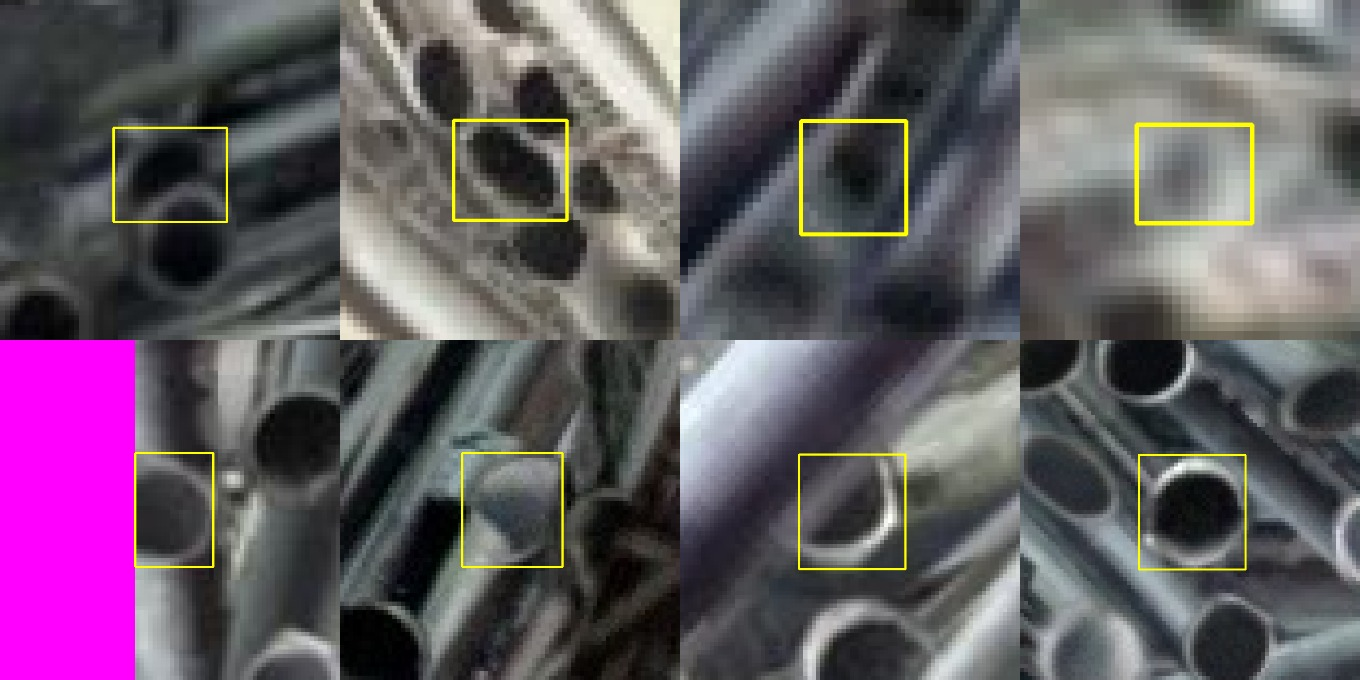
\includegraphics[width=\textwidth]{abbildungen/label_check.jpg}
\caption[Kontrolle der Labelerzeugung]{Kontrolle der Labelerzeugung. Die Boxen
umschließen den \emph{sichtbaren} Umriss; stark verdeckte Instanzen erhalten
kein Label und bleiben damit als hartes Negativ im Bild.}
\label{abb:labelcheck}
\end{figure}

\subsection{T8 -- Globale Bildstufe}
\label{sec:globalstufe}

Die letzte Stufe wirkt auf das \emph{gesamte} Bild. Das ist entscheidend: Nur
eine bildweite Operation kann eine Signatur vereinheitlichen, die zwischen
Objekt und Hintergrund unterscheidbar wäre.

\begin{table}[htbp]
\centering
\caption[T8: Globale Bildstufe]{T8 -- globale Bildstufe. \emph{Ist} = gemessener
Anteil je Bild.}
\label{tab:t8}
\footnotesize
\begin{tabularx}{\textwidth}{@{}L{0.20\textwidth}L{0.07\textwidth}XL{0.045\textwidth}@{}}
\toprule
\textbf{Transformation} & \textbf{Ist} & \textbf{Begründung} & \textbf{Art} \\
\midrule
Helligkeit/Kontrast & 89{,}6\,\% &
Wetter- und Belichtungsvariation ($\times 0{,}80$--$1{,}22$, Offset
$\pm 18$ Grauwerte). & M \\
HSV / Farbtemperatur & 69{,}0\,\% &
Bewölkt (blaustichig) bis Abendsonne (warm). Alle vier Clean Plates sind bei
diffusem Licht aufgenommen -- diese Stufe ist der einzige Ersatz für die
fehlende Beleuchtungsvielfalt und damit eine bewusste Approximation. & A \\
Defokus ($\sigma$ 0,3--1,0\px) & 34{,}4\,\% &
Der Autofokus trifft bei Stapelaufnahmen oft die falsche Ebene. & L \\
Bewegungsunschärfe & 9{,}9\,\% &
Verwacklung aus der Hand; Baustellenaufnahmen entstehen im Vorbeigehen.
Niedriger Anteil, weil moderne Mobiltelefone kurz belichten. & A \\
Sensorrauschen & 80{,}1\,\% &
Vereinheitlicht das Rauschniveau über das ganze Bild
($\sigma = 1{,}0$--$5{,}0$). & L \\
Vignettierung & 25{,}0\,\% &
Weitwinkelobjektive von Mobiltelefonen; erzwingt zusätzlich
Positionsinvarianz der Helligkeit. & L \\
JPEG-Requantisierung $q \in [55, 95]$ & 85\,\% (Soll) &
\textbf{Die wichtigste unsichtbare Transformation} (Signatur~S5). Eingeklebte
Pixel behalten sonst eine andere DCT-Blockstatistik als der Hintergrund, der
bereits einmal komprimiert war \parencite{wallace1992jpeg}. Ein erneuter
Kompressionsdurchlauf über das Gesamtbild vereinheitlicht diese Signatur. Sie
ist forensisch die belastbarste Einfügemarke überhaupt \parencite{farid2009} --
wer sie stehen lässt, liefert dem Netz eine perfekte Abkürzung. & L \\
\bottomrule
\end{tabularx}
\end{table}

\subsection{T9 -- Negativbilder}
\label{sec:negative}

9,7\,\% der erzeugten Bilder enthalten \emph{kein} Objekt: Rohrstapel ohne
Stirnflächen, Kieswerk, Betondeck mit Maschendrahtzaun.

Die Begründung folgt direkt aus der Annotationsdefinition
(Abschnitt~\ref{sec:annotation}): Die dominante Falschpositiv-Quelle in dieser
Domäne sind Rohrschäfte, Gitterknoten und dunkle Löcher im Maschendraht -- alles
Strukturen, die den Stirnflächen ähneln, aber ausdrücklich keine Objekte sind.
Explizite Negativbilder bestrafen genau diese Verwechslung; sie sind das
statische Gegenstück zum Hard-Example-Mining
\parencite{shrivastava2016}. Der Anteil von rund 10\,\% entspricht der Empfehlung
der verwendeten Werkzeugkette \parencite{ultralyticsdocs}; ein höherer Anteil
würde den Anteil positiver Gradienten unnötig verdünnen.

\section{Der erzeugte Datensatz}
\label{sec:datensatz}

\begin{table}[htbp]
\centering
\caption[Kenngrößen des erzeugten Datensatzes]{Kenngrößen des erzeugten
Trainingsdatensatzes.}
\label{tab:datensatz}
\small
\begin{tabular}{@{}lr@{}}
\toprule
Bilder ($1024\times1024$) & 6\,000 \\
davon Negativbilder & 583 \quad (9{,}7\,\%) \\
gerenderte Instanzen & 173\,100 \\
\textbf{gelabelte Objekte} & \textbf{136\,384} \quad (22{,}7 pro Bild) \\
verworfen (Verdeckung / Rand / Größe) & 34\,875 \quad (20{,}1\,\%) \\
mittlere Sichtbarkeit der gelabelten Objekte & 90{,}0\,\% \\
teilverdeckte gelabelte Objekte & 30{,}1\,\% \\
Objektdurchmesser p05 / Median / p95 & 11{,}6 / 22{,}5 / 39{,}9\px \\
Seitenverhältnis p10 / Median / p90 & 0{,}77 / 1{,}00 / 1{,}40 \\
Objekte pro Bild p05 / Mittel / p95 & 0 / 22{,}7 / 64 \\
\bottomrule
\end{tabular}
\end{table}

\subsection{Kalibrierungsnachweis}
\label{sec:kalibrierung}

Der wichtigste Qualitätsnachweis der Pipeline ist nicht der optische Eindruck,
sondern der Vergleich der erzeugten Statistik mit der gemessenen realen
Statistik. Tabelle~\ref{tab:kalibrierung} stellt beide gegenüber.

\begin{table}[htbp]
\centering
\caption[Kalibrierung gegen die Realmessung]{Kalibrierung des Layoutmodells
gegen die Realmessung ($n = 174$ reale Labels). Alle Abstände in
Objektdurchmessern.}
\label{tab:kalibrierung}
\footnotesize
\begin{tabular}{@{}lccc@{}}
\toprule
\textbf{Kenngröße} & \textbf{real \code{val}} & \textbf{real \code{test}} &
\textbf{synthetisch (Ist)} \\
\midrule
NN-Abstand p10 / Median / p90 & 0{,}86 / 1{,}09 / 1{,}78 &
0{,}83 / 1{,}24 / 2{,}51 & \textbf{0{,}84 / 1{,}17 / 1{,}87} \\
berührt den NN ($< 1{,}2\,\Oe$) & 61{,}4\,\% & 46{,}5\,\% & \textbf{53{,}6\,\%} \\
Nachbarn innerhalb $5\,\Oe$ (Median) & 10 & 10 & \textbf{13} \\
Größenverhältnis zum NN (Median) & 1{,}05 & 1{,}05 &
\textbf{1{,}05}$^{*}$ \\
\bottomrule
\multicolumn{4}{@{}l@{}}{\footnotesize $^{*}$ per Konstruktion, siehe Gleichung~\eqref{eq:layout}} \\
\end{tabular}
\end{table}

Die synthetische Verteilung liegt bei allen vier Kenngrößen zwischen oder nahe
bei den beiden realen Messungen. Die einzige systematische Abweichung ist die
Nachbarzahl: Die synthetischen Cluster sind im Mittel etwas dichter als die
realen (13 statt 10 Nachbarn innerhalb $5\,\Oe$, im Maximum 61 statt 20). Das
ist bewusst so belassen -- eine höhere Dichte im Training ist eine
Robustheitsreserve, weil sie den Detektor auf schwierigere Szenen vorbereitet als
die, die er zur Inferenzzeit vorfindet. Die umgekehrte Abweichung wäre
gefährlich gewesen.

\begin{figure}[htbp]
\centering
\begin{subfigure}{0.32\textwidth}
  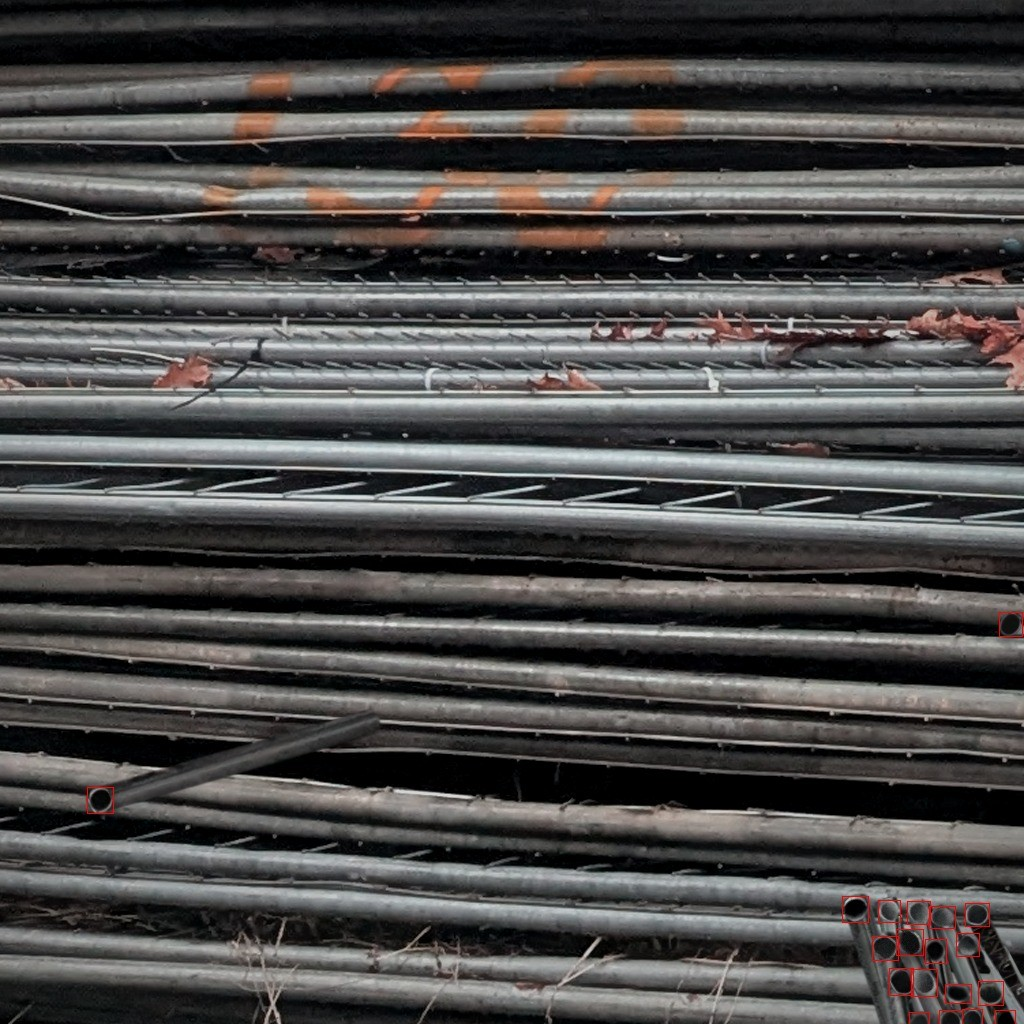
\includegraphics[width=\textwidth]{abbildungen/synth_000.jpg}
\end{subfigure}\hfill
\begin{subfigure}{0.32\textwidth}
  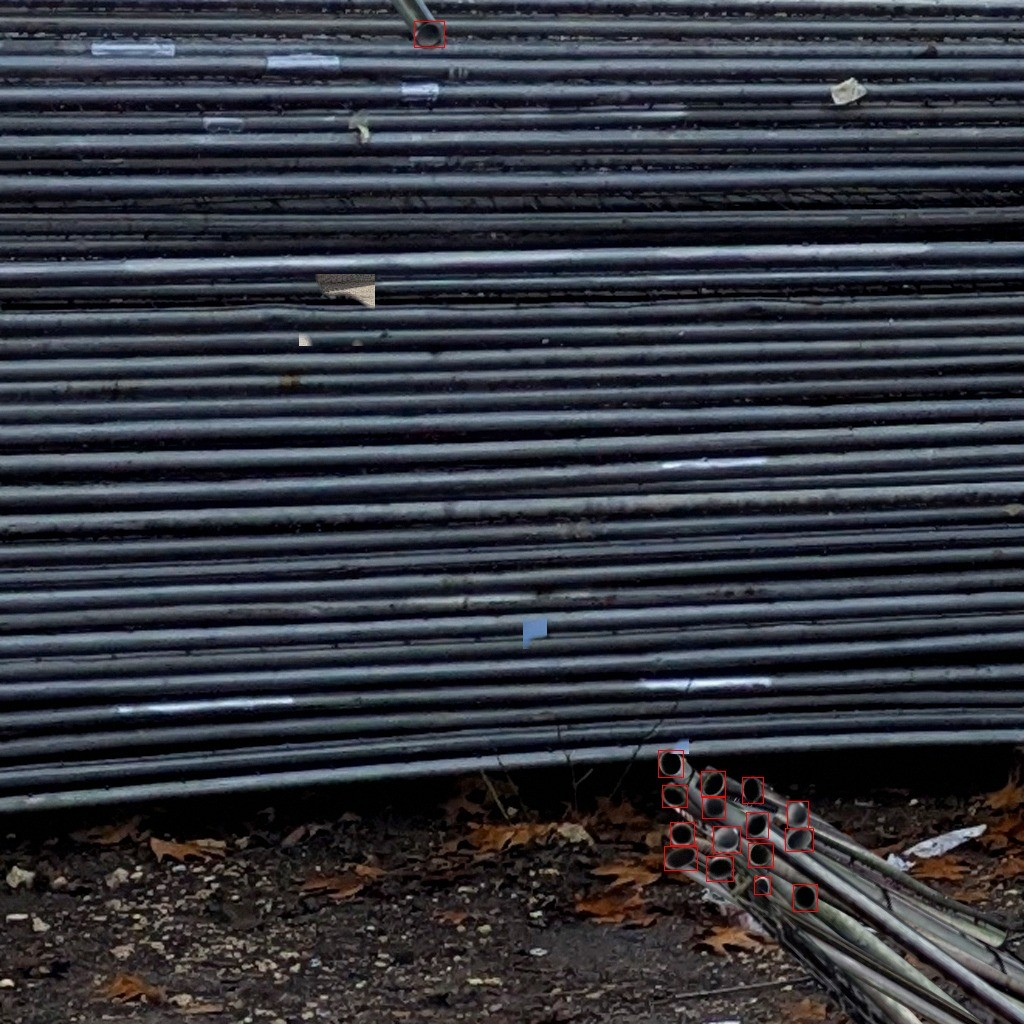
\includegraphics[width=\textwidth]{abbildungen/synth_001.jpg}
\end{subfigure}\hfill
\begin{subfigure}{0.32\textwidth}
  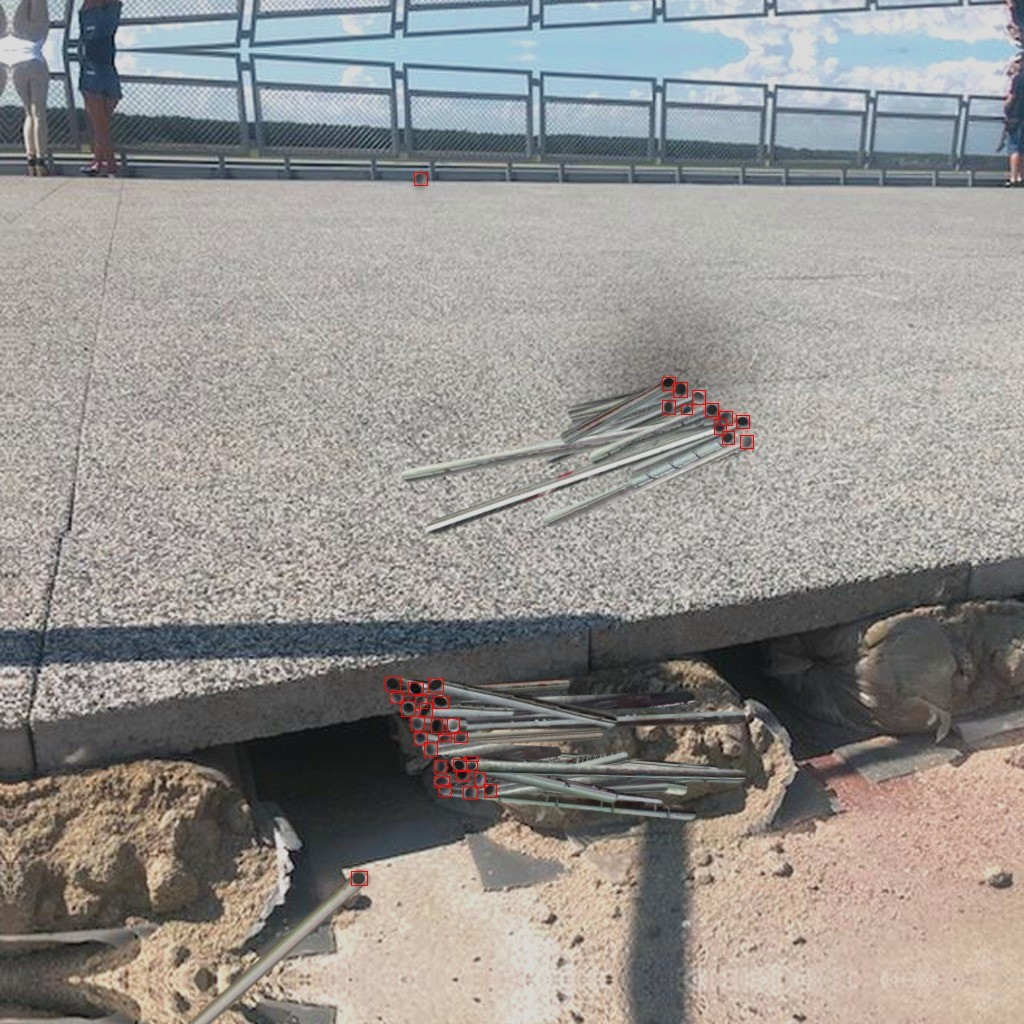
\includegraphics[width=\textwidth]{abbildungen/synth_002.jpg}
\end{subfigure}

\vspace{2mm}
\begin{subfigure}{0.32\textwidth}
  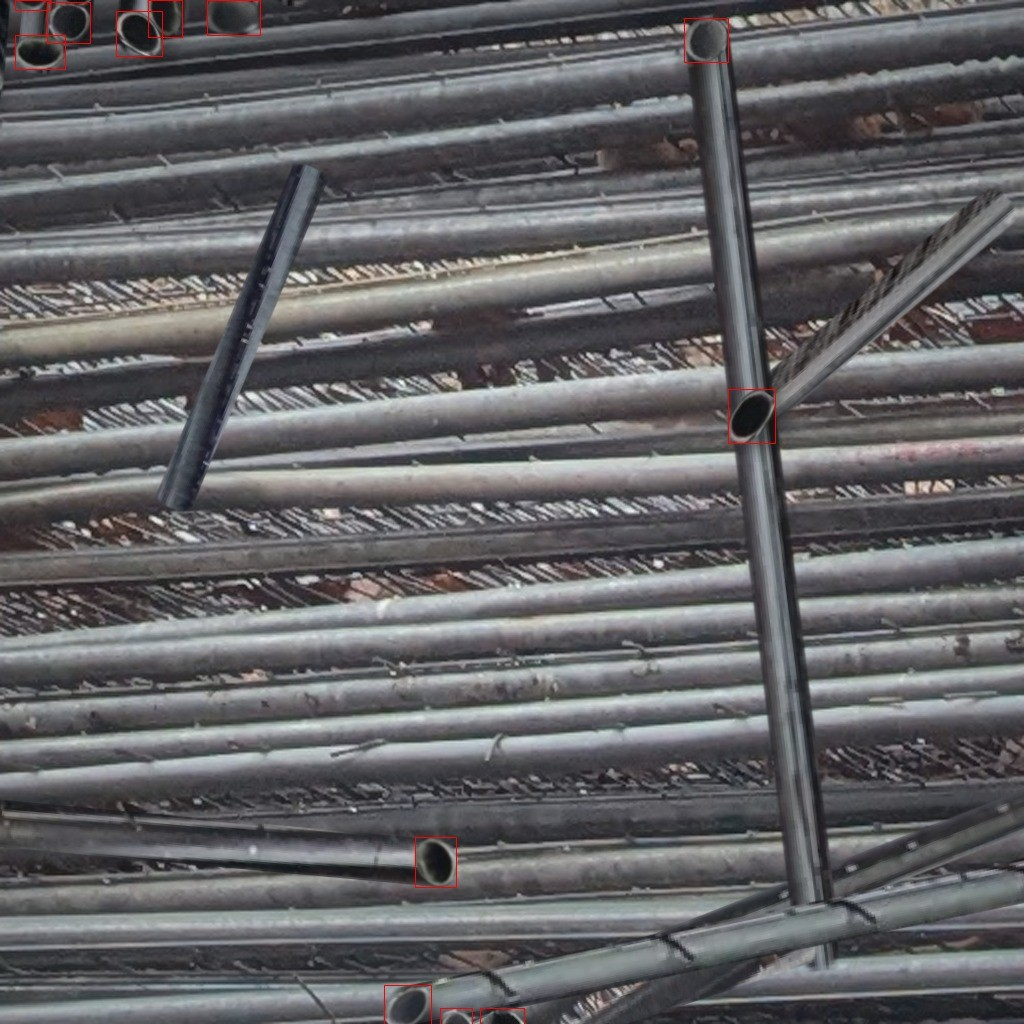
\includegraphics[width=\textwidth]{abbildungen/synth_003.jpg}
\end{subfigure}\hfill
\begin{subfigure}{0.32\textwidth}
  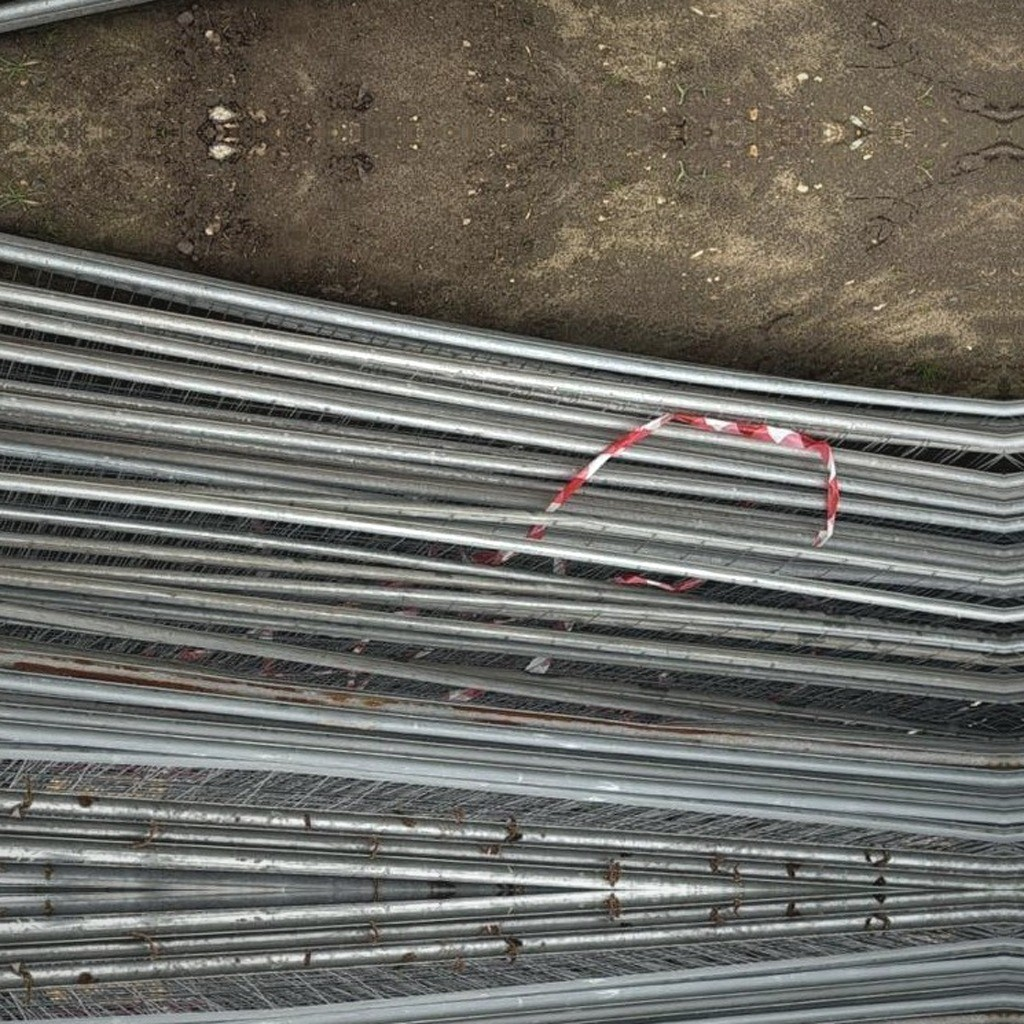
\includegraphics[width=\textwidth]{abbildungen/synth_004.jpg}
\end{subfigure}\hfill
\begin{subfigure}{0.32\textwidth}
  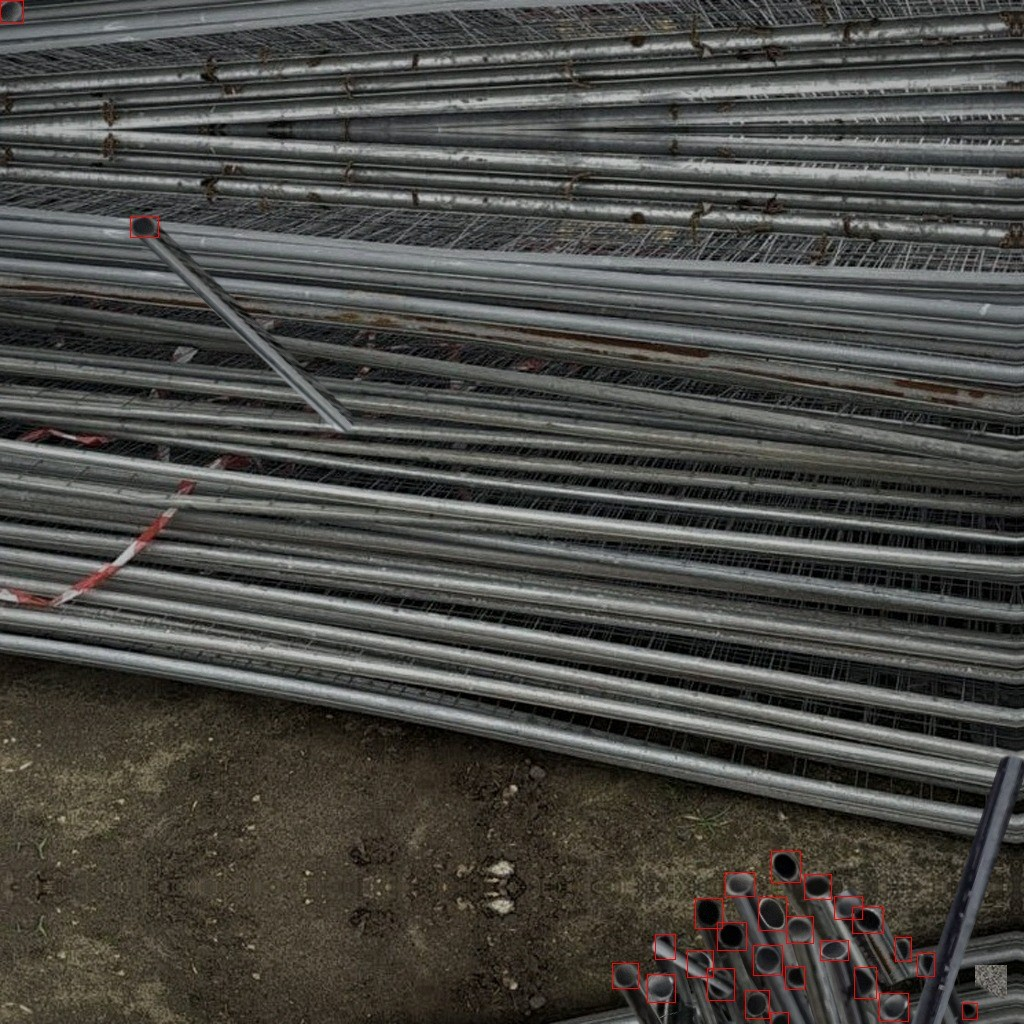
\includegraphics[width=\textwidth]{abbildungen/synth_005.jpg}
\end{subfigure}
\caption[Beispiele synthetischer Trainingsbilder]{Sechs synthetische
Trainingsbilder mit eingezeichneten erzeugten Labels. Erkennbar sind die
Clusterstruktur des Layoutmodells, die Rohrschäfte hinter den Stirnflächen, die
quer liegenden Okkluder und die abgedunkelten Mulden. Am unteren Rand des
mittleren Bildes der unteren Reihe ist die in
Abschnitt~\ref{sec:grenzen} genannte Spiegelsymmetrie des Reflect-Paddings
sichtbar.}
\label{abb:synthbeispiele}
\end{figure}

\section{Nachweis der Anforderungen}
\label{sec:nachweis}

Tabelle~\ref{tab:nachweis} prüft die in Abschnitt~\ref{sec:anforderungen}
aufgestellten Anforderungen gegen die umgesetzte Pipeline.

\begin{table}[htbp]
\centering
\caption[Nachweis der Anforderungen A1--A6]{Nachweis der Anforderungen aus
Abschnitt~\ref{sec:anforderungen}.}
\label{tab:nachweis}
\footnotesize
\begin{tabularx}{\textwidth}{@{}L{0.07\textwidth}XL{0.12\textwidth}@{}}
\toprule
\textbf{Anf.} & \textbf{Umsetzung} & \textbf{Status} \\
\midrule
A1 & Box wird nach jeder Instanztransformation aus der transformierten
Alphamaske neu bestimmt; \code{degrees}, \code{shear}, \code{perspective} zur
Trainingszeit auf 0 & erfüllt \\
A2 & Objektgrößen 12--44\px{} aus der Realmessung; Leinwand
$1024 = $ \code{imgsz}, also keine Skalierung im Training & erfüllt \\
A3 & Zoom an Rohrdurchmesser gekoppelt; Schaft hinter jeder Stirnfläche;
parallele Schaftrichtung; Tiefenmodell 75/25; Rotation voll, weil physikalisch
unbeschränkt & erfüllt \\
A4 & S1 Alphamaske + Kantenweichzeichnung; S2 partieller Farbangleich; S3
flächentreue Skalierung + Unschärfeangleich; S4 lokal geschätzter Rauschangleich;
S5 JPEG-Requantisierung; S6 Schlagschatten + physikalische Verdeckung & erfüllt \\
A5 & modale Boxen; Verwerfen unter 30\,\% Sichtbarkeit bzw.\ 15\,\%
Bildanteil -- dieselben Regeln wie bei der Handannotation & nur annähernd
erfüllt: Restversatz der Boxgröße 1,2--2,5\px{}
(Abschnitt~\ref{sec:boxversatz}) \\
A6 & 36 Transformationen mit Soll-Bereich und gemessenem Ist-Anteil
(Tabellen~\ref{tab:t1}--\ref{tab:t8}); sechs Werte ausdrücklich als Annahme
gekennzeichnet & erfüllt \\
\bottomrule
\end{tabularx}
\end{table}

Die Anforderungen sind damit formal erfüllt. Das sagt allerdings nichts darüber
aus, ob die einzelnen Maßnahmen \emph{wirken} -- Erfüllung einer
Entwurfsanforderung ist kein empirischer Nachweis. Diese Unterscheidung wird in
Kapitel~\ref{kap:auswertung} durch die Messung des Sim-to-Real-Abstands und die
Okklusionsablation adressiert und in Abschnitt~\ref{sec:tragend} explizit
bilanziert.
